\section{Resultados e Discussão}

Os resultados obtidos demonstram ser possível embarcar PIRNNs em plataformas de baixo custo com eficiência e robustez. Essa compatibilidade torna essa abordagem particularmente atrativa para aplicações industriais e acadêmicas que possuem restrições orçamentárias, permitindo a implementação de soluções de controle e simulação em larga escala sem a necessidade de hardware especializado ou de alto custo. Outro fator positivo foi o espaço ocupado pelo programa: verificou-se que o programa completo, que inclui tanto o modelo quanto o código responsável pela comunicação serial com o computador, utilizou apenas 68,4\% da memória flash e 13,2\% da memória RAM do Arduino. Esses números indicam que existem recursos disponíveis para implementação de modelos mais complexos ou execução de tarefas adicionais, caso necessário.

Nos testes de robustez, foram simulados cenários com ruído nas medições e com ausência completa de medições. A Figura \ref{fig:sil-pirnn} apresenta os resultados obtidos nesses testes. Observa-se que, no caso de medições ruidosas, o modelo capta as variações impostas pelo ruído, mas com um leve amortecimento, sugerindo uma capacidade de filtragem parcial das perturbações. Quando as medições são interrompidas completamente, o modelo passa a se retroalimentar. Nesse cenário, o modelo continua seguindo com precisão o comportamento esperado dos tanques, mesmo sem a entrada de dados dos sensores.

% Local original da figura fig:sil-pirnn

Nos testes de desempenho, a PIRNN demonstrou uma significativa vantagem em termos de velocidade quando comparada com métodos numéricos tradicionais. A comparação foi feita com os métodos RK, CVODES e IDAS da biblioteca \textit{CasADi}, e os métodos RK45, RK23 e LSODA da biblioteca \textit{SciPy}, todos executados no mesmo computador. Para avaliar o desempenho de cada método, foram realizadas 100 medições do tempo necessário para simular aproximadamente 33 horas de operação, considerando intensas perturbações na vazão de entrada. A Figura \ref{fig:pirnn-benchmark-lite} apresenta o boxplot dos tempos de execução dos métodos avaliados, evidenciando a superioridade da PIRNN em termos de tempo de processamento.

\begin{figure}[ht]
  \centering
  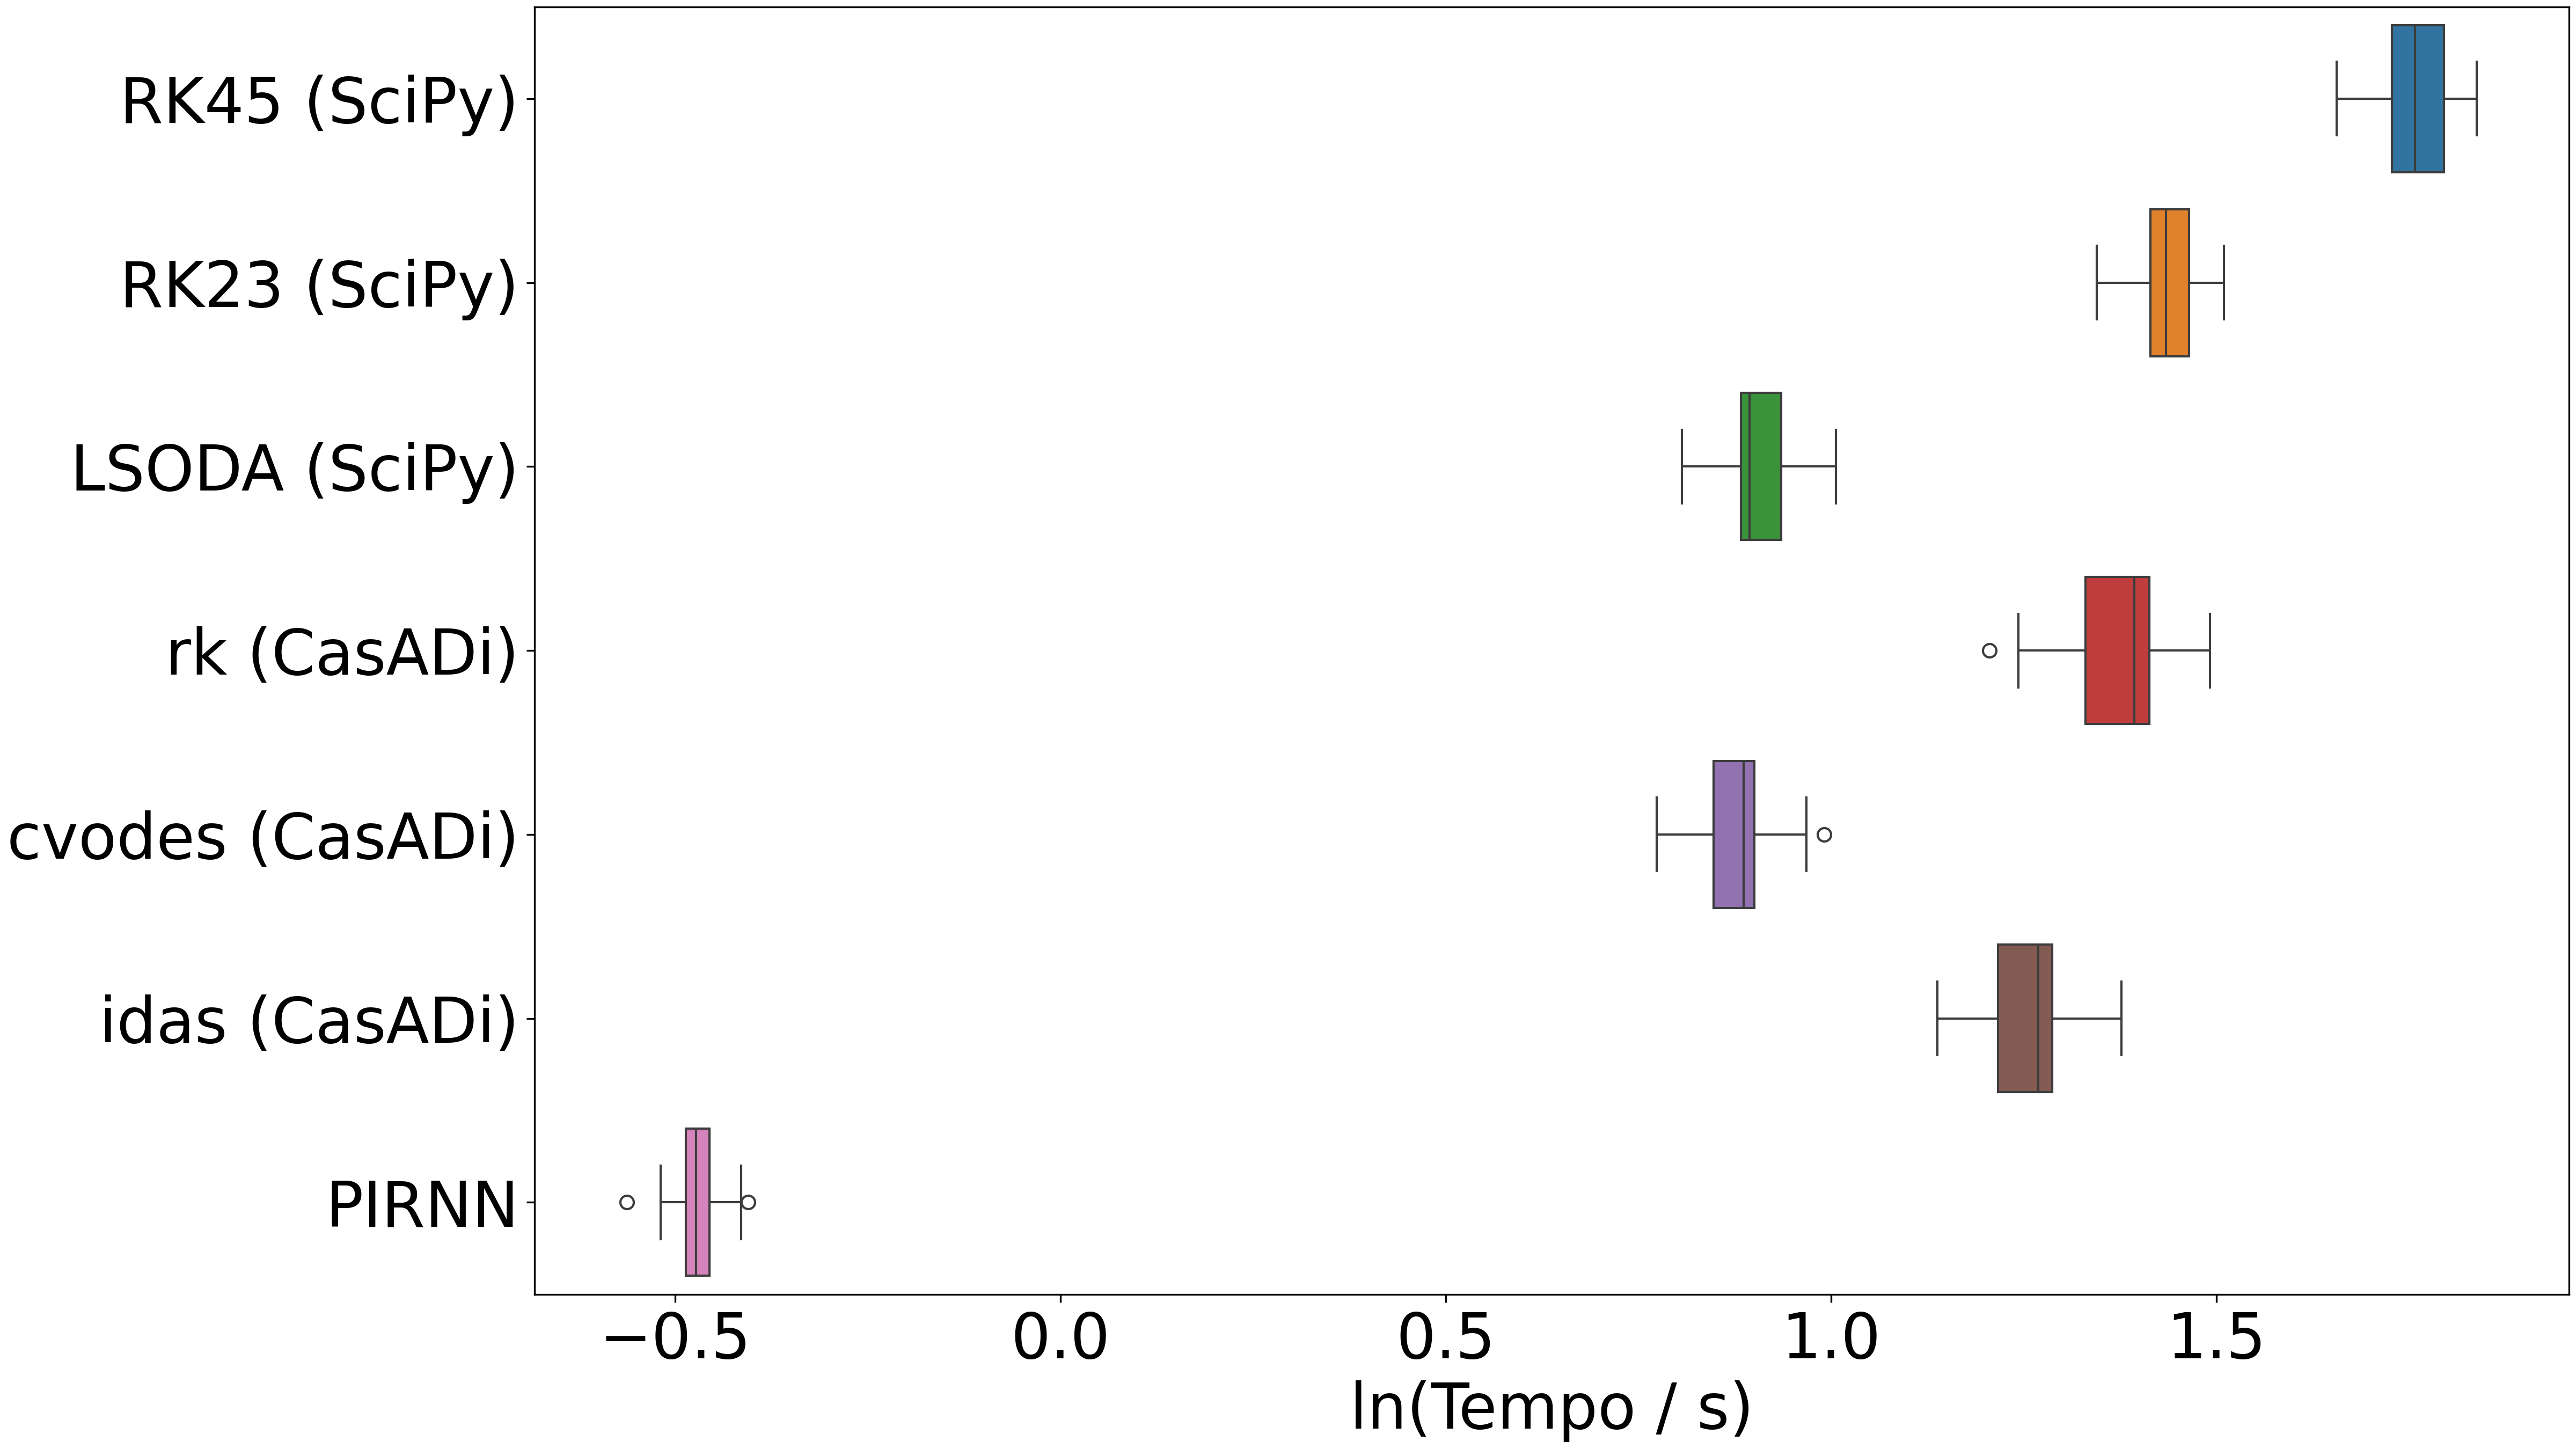
\includegraphics[width=0.45\textwidth]{pirnn-boxplot.png}
  \caption{Boxplot dos tempos de execução em escala de logaritmo natural dos métodos avaliados.}
  \label{fig:pirnn-benchmark-lite}
\end{figure}

Esses resultados mostram que o uso de PIRNNs embarcadas pode ser uma alternativa viável aos métodos tradicionais na simulação e controle de sistemas. A arquitetura proposta mostrou-se capaz de fornecer respostas rapidamente, o que é essencial para aplicações de controle em tempo real. Além disso, os testes de robustez demonstraram que a PIRNN manteve a qualidade das previsões mesmo em cenários adversos, como a presença de ruídos ou ausência de medições.
